\chapter{Introduction}

This initial section of this chapter will mostly serve as a historical overview of the field of particle physics, leading to the development of the \textbf{Standard Model}--the theory that describes all of the fundamental\footnote{As of the year 2023, but reading this chapter will hopefully illustrate why this may be subject to change in the (likely very distant) future.} particles and the way in which they interact with each other. An emphasis will be made on the discovery of quarks, as the research presented in this thesis is centered around these particles. This section will contain little-to-no mathematics, as historical lessons generally do not. 

The second section will more thoroughly introduce the Standard Model, and how it was developed from a theoretical perspective. Words like ``fundamental representation'' and ``gauge symmetry'' will be thrown around, but the goal is to provide a high-level mathematical overview of the theory and how it was developed without getting bogged down in the details.

As this thesis is focused nearly entirely on the strong nuclear force, the remaining sections of the chapter will delve into the details of Quantum ChromoDynamics (QCD), which is the component of the Standard Model which describes the interactions between \textbf{quarks} and \textbf{gluons}--the consituent particles of the more familiar protons and neutrons. Unfortunately, QCD is enormously complicated and the full theory is not yet fully understood. While this may be disheartening for theorists, it is a boon for experimentalists as it provides a wealth of opportunities to probe the theory in regimes where it is both understood and not understood. 

To that end, the remainder of the chapter will focus on the ways in which QCD can be investigated using heavy-ion collisions, with an emphasis on the \textbf{Quark-Gluon Plasma} (QGP)--a novel state of nuclear matter that QCD predicts should exist at the extreme temperatures and densities that are achieved in these collisions. The experimental signatures of QGP formation will also be discussed, with a particular focus on \textbf{strangeness enhancement}--the phenomenon where the production of strange quarks is enhanced in heavy-ion collisions relative to proton-proton collisions. 

\section{What is fundamental?}
The answer to the question ``What are the fundamental building blocks of our universe?'' has changed drastically over the course of human history. The idea that all matter is composed of smaller, uncuttable pieces has been around since 5th century BCE when Greek philosophers Democritus and Leucippus first introduced the concept of an atom~\cite{GreekAtom}. While this idea was mostly motivated by philosophical reasoning, it was later adopted by the English scientist John Dalton in the 19th century to explain the results of his chemical experiments, where he found that chemical elements always combined with each other by discrete units of mass~\cite{Dalton}. As scientists discovered more and more of these elements, the number of ``fundamental'' building blocks grew as well. By the late 1800s, over 70 unique chemical elements had been discovered, though they would often be grouped together due to similar chemical properties using what chemist Dimitri Mendeleev dubbed the \textit{periodic table of elements}~\cite{PeriodicTable}. An example of the periodic table from the time of Mendeleev can be seen in Figure~\ref{fig:periodic_table}. While this grouping was useful for chemists, it also served as a hint to physicists that perhaps these elements were not actually fundamental, but rather composed of even smaller pieces.

\begin{figure}[ht]
    \centering
    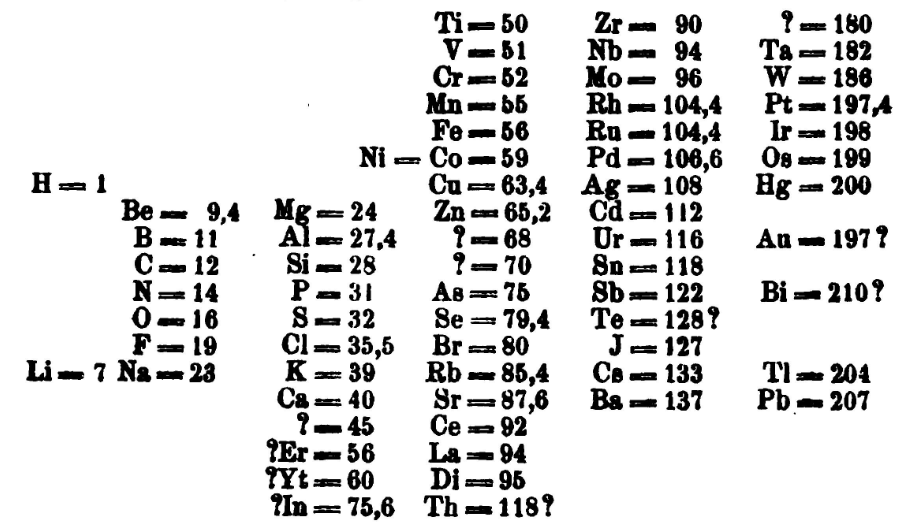
\includegraphics[width=0.7\textwidth]{figures/introduction/PeriodicTable.png}
    \caption{Dimitri Mendeleev's periodic table of elements from the late 1800s, taken from~\cite{MendeleevPaper}. The elements are grouped by similar chemical properties, and the gaps in the table are where Mendeleev predicted that new elements would be discovered.}
    \label{fig:periodic_table}
\end{figure}


Things changed quite a bit around the turn of the 20th century, with scientists like Rutherford and Chadwick determining that the supposedly indivisible atom was composed of even smaller sub-atomic particles, eventually named electrons, protons and neutrons~\cite{Electrons, Protons, Neutrons}. Thus the number of fundamental blocks of matter had decreased substantially from nearly 100 to just three, but only very briefly. Only months after the discovery of the neutron, the fundamental anti-particle of the electron--known as the positron--was discovered in 1932 by Carl Anderson~\cite{Positron}. In the next two decades, the number of known fundamental particles would skyrocket. In 1947, the muon was discovered~\cite{Muon}, followed by the discovery of a laundry list of particles~\cite{Kaon,Lambda,Sigma} that participate in the same interaction that holds oppositely charged protons together in the nucleus of an atom--the so-called \textbf{strong nuclear force}. These ``fundamental'' particles were collectively called \textbf{hadrons}, which were further separated into lighter and heavier categories dubbed \textbf{mesons} and \textbf{baryons}, respectively~\cite{MesonBaryon}. By the late 1960s, the number of known hadrons had grown to well over 100~\cite{ParticleDiscoveries}, which is a far cry from the number of ``fundamental'' chemical elements that were known to exist in the 1800s.

In the same way that Mendeleev tried to group the elements by their similar chemical properties, physicists attempted to group the hadrons together based on their known sub-atomic properties at the time. The first successful attempt at such a grouping was the \textbf{Eightfold Way}, which was independently proposed by Murray Gell-Mann and Yuval Ne'eman in 1961~\cite{GellMannEightfold, NeemanEightfold}. This grouping was found by examining the following properties of the hadrons:
%
\begin{enumerate}
    \item \textbf{Isotopic spin}: a quantum number introduced by Werner Heisenberg in 1932 to try to explain the apparent symmetries between the proton and neutron with respect to the strong nuclear force~\cite{IsotopicSpin} (i.e. although the proton and neutron have different electric charges, the strong interaction does not seem to distiguish between the two)
    \item \textbf{Strangeness}: another quantum number introduced by Gell-Mann and Nishijima in 1953 to explain why some hadrons decayed much more slowly than expected, but such particles appeared to be created in pairs~\cite{Strangeness}. In other words, the strong interaction responsible for the creation of these particles appeared to conserve strangeness, but the weak interaction responsible for the slower decay of these particles did not. This\footnote{Strangeness was introduced a few years before the very first quark model, but it now has the modern interpretation which is directly related to the number of strange and anti-strange quarks within a hadron.} quantity is of utmost importance to this thesis, and will be discussed in much greater detail in the coming sections.
\end{enumerate}
%
\begin{figure}[t!]
    \centering
    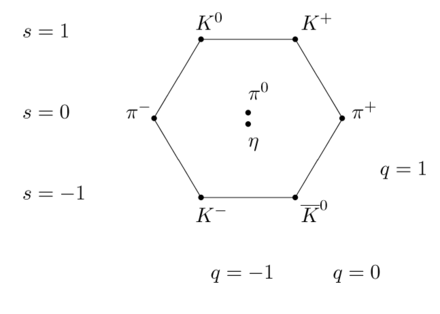
\includegraphics[width=0.49\textwidth]{figures/introduction/Meson_octet.png}
    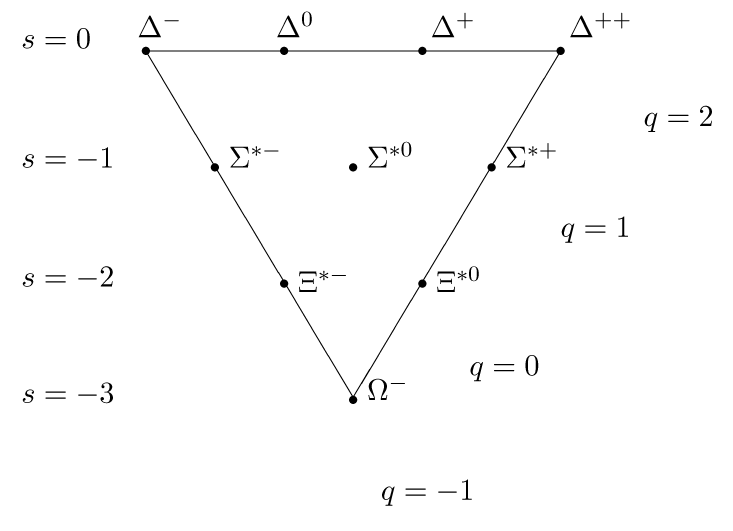
\includegraphics[width=0.49\textwidth]{figures/introduction/Baryon_decuplet.png}
    \caption{The ``Eightfold Way'' diagrams of the J = 1/2 mesons (left) and J = 3/2 baryons (right) plotted against strangeness and electric charge. Understanding the underlying symmetry group that gives rise to such patterns\protect\footnotemark \  ultimately led to the development of the quark model. While the original patterns were found using isotopic spin and hypercharge, it is trivial to convert between the two using the Gell-Mann-Nishijima formula~\cite{GellMannNishijima_1, GellMannNishijima_2}.}
    \label{fig:eightfold_way}
\end{figure}
\footnotetext{Namely SU(3), but this is a history lesson. Also the path from SU(3) to patterns of this type is long and arduous, involving a thorough understanding of representation theory.}
%
Plotting the baryons and mesons in a two-dimensional space based on these two properties revealed striking patterns, as shown in Figure~\ref{fig:eightfold_way}. Similar to Mendeleev, GellMann also left a blank space\footnote{The original paper on the Eightfold Way does not contain any of these diagrams, but there are discussions about the properties of particles that should exist if the theory were correct, but had not been observed~\cite{GellMannEightfold}.} where he believed a new particle--the $\Omega^{-}$--would be discovered.  The patterns in these diagrams hinted at an underlying symmetry governing the strong nuclear force, and ultimately led to the invention of the very first quark model by Gell-Mann and Zweig in 1964~\cite{QuarkModel}. This model proposed that all of the hadrons were actually composed of even smaller particles, which Gell-Mann dubbed ``quarks''. The quark model was able to explain the patterns seen in Figure~\ref{fig:eightfold_way} by introducing three different types of fermionic quarks--up, down and strange--along with their corresponding anti-quarks. Baryons would then be composed of three such quarks, whereas mesons would be composed of quark and anti-quark pairs. If the quark model were correct, the number of fundamental building blocks of matter would again decrease from over 100 to just 14: electrons, muons, electron neutrinos, muon neutrinos, up quarks, down quarks, strange quarks, and all of their corresponding anti-particles.


Initially, many physicists believed that the quarks from this model were just a mathematical abstraction~\cite{QuarkAbstraction}. This possibility did not stop Sheldon Glashow and James Bjorken from extending the quark model in less than a year after its inception by introducing a fourth quark: the charm~\cite{CharmQuark}. This new quark was primarily introduced to equalize the number of leptons (four at the time: electron, muon, and their respective neutrinos) with the number of quarks. The theory was mostly aesthetic~\cite{AestheticCharm} in that the charm quark was not explicity required by any known mechanisms. It was only after the Glashow-Iliopoulos-Maiani (GIM) mechanism was introduced in 1970~\cite{GIM} that the existence of the charm quark became ``necessary''. This mechanism helped explain why neutral kaons decayed into two muons at a much lower rate than expected, but it required the existence of a quark with the same charge as the up quark but with a much larger mass.

On the experimental side of things, the notion that protons and neutrons were fundamental particles was also being challenged. The deep inelastic scattering experiments at the Standford Linear Accelerator Center (SLAC) performed by Kendall, Friedman and Taylor in 1968~\cite{Kendall, Friedman, Taylor} revealed unexpected\footnote{Depending on who you asked at the time, both the three and four quark models were not universally accepted.} behavior when probing the structure of the proton: it appeared to be composed of point-like particles. These experiments were performed by firing electrons at stationary protons and measuring the energy distributions of the scattered electrons at different scattering angles. An example such a distribution for electrons with initial energies of 10 GeV scattered at 6 degrees can be seen in Figure~\ref{fig:dis}. The large spike on the left side of the distribution corresponds to the elastic scattering of the electron off the proton, which was well understood at the time~\cite{ElasticScattering}. The ``bumps'' observed at lower values of the scattered electron energy were also well understood~\cite{Resonances}, and they correspond to the ``shallow'' inelastic scattering of the electron off the proton, where the proton gets excited into a so-called \textit{resonance} state (like the $\Delta$ baryon). However, the ``background'' underneath the bumps and the apparent continuum of events at even lower values of the scattered electron energy correspond to a mess of unknown particles being produced. This mess of particles appeared to grow with increasing scattering angle and decreasing scattered electron energy, which ultimately led to the conclusion that the proton was composed of point-like particles that were being ``knocked out'' of the proton by the incoming electron~\cite{Kendall, BjorkenScaling}.

\begin{figure}[ht]
    \centering
    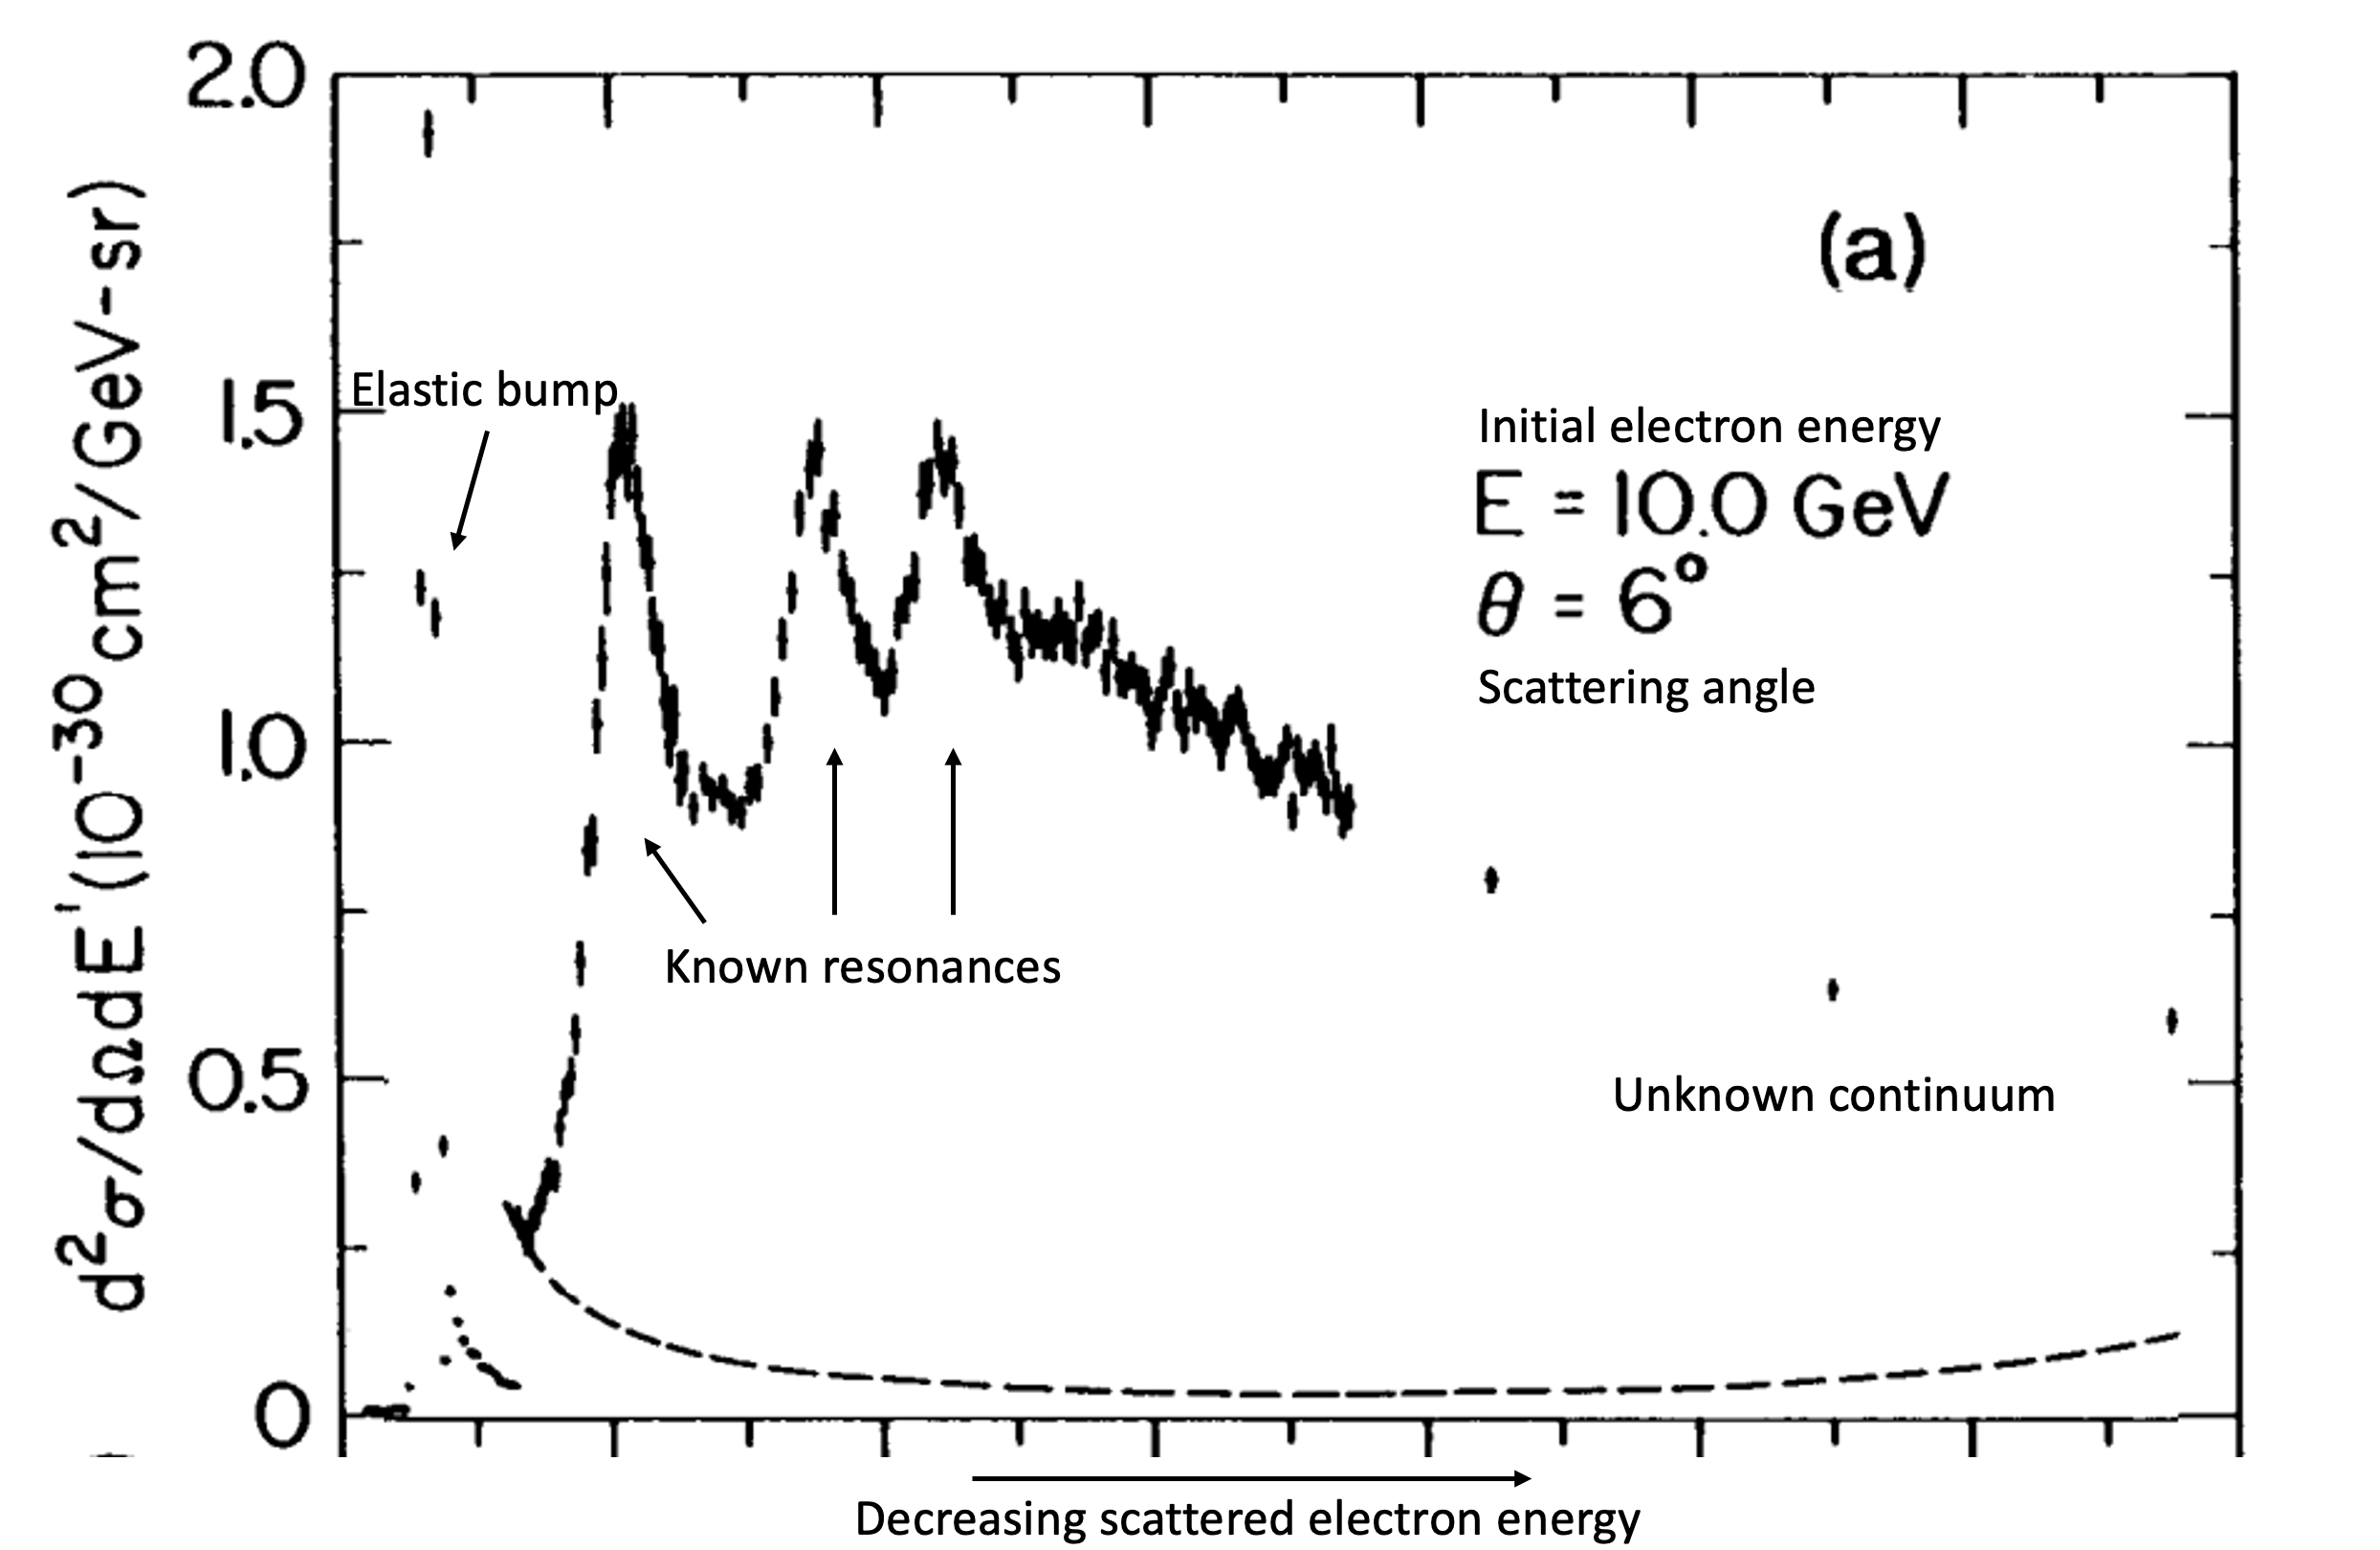
\includegraphics[width=0.7\textwidth]{figures/introduction/DeepInelasticScattering.png}
    \caption{The energy distribution of electrons scattered off of protons at an initial electron energy of 10 GeV and a scattering angle of 6 degrees. The large spike on the left side of the distribution corresponds to the elastic scattering of the electron off the proton, and the ``bumps'' correspond to the inelastic scattering of the electron off the proton. The ``background'' underneath the bumps and the apparent continuum of events at even lower values of the scattered electron energy correspond to a mess of unknown particles being produced. The behavior of this continuum with respect to the scattering angle and the scattered electron energy ultimately led to the conclusion that the proton was not fundamental.}
    \label{fig:dis}
\end{figure}

While many physicists were perfectly happy to interpret these point-like particles as the very same quarks from the aforementioned quark model(s), they received the much more noncommittal name \textbf{partons} after Richard Feynman's parton model of hadrons~\cite{Partons}. The association of these partons with quarks was not universally accepted\footnote{No acceptance of any model is a step function, but the discovery of J/$\psi$ seems to be a turning point in literature.} until the discovery of the J/$\psi$ meson in 1974~\cite{Jpsi}. In the meantime, the theoretical description of the strong nuclear force was closing in on its final form. The formulation of Quantum ChromoDynamics (QCD) in the early 1970s by Gell-Mann, Fritzsch, and Leutwyler~\cite{QCDFormulation} resolved many of the issues that were present in the initial quark models\footnote{For example, the wavefunction of the $\Delta^{++}$ baryon under the first quark model was not anti-symmetric, which is a requirement for fermions.}. QCD introduced the concept of color charge, which all of the quarks would carry. The mediating bosons of the strong interaction--known as \textbf{gluons}--were also introduced\footnote{And also carried color charge, but more details will be discussed in Section~\ref{sec:qcd}}. 

While QCD gave a solid mathematical description of the strong interaction, it wasn't until the discovery of \textbf{asymptotic freedom}~\cite{AssFreedom1, AssFreedom2} by Gross, Wilczek and Politzer in 1973 that the theory became experimentally testable. Asymptotic freedom is the notion that the strong interaction becomes weaker at higher energies, allowing for QCD calculations to be performed using perturbative techniques. This discovery allowed theorists to use QCD to make predicitions of the results of very high energy particle collision experiments. The first QCD prediction to be experimentally verified came from the Positron-Electron Tandem Ring Accelerator (PETRA) in 1979~\cite{PETRA}, which experimentally confirmed the existence of gluons~\cite{GluonConfirmation}. With experimental verification of QCD, it became clear that the association of partons with quarks was indded incorrect: they are both quarks \textit{and} gluons.

While not of particular import to this thesis\footnote{Though extremely interesting in its own right}, the theory of electroweak interactions was also being developed during the 1960s by Glashow, Weinberg and Salam~\cite{Electroweak1, Electroweak2}. With this new theory came the prediction of four\footnote{The Higgs mechanism (which predicts the existence of the Higgs boson) came before electroweak unification~\cite{HiggsPaper}, but it was a requirement for the theory.} new bosons: the Higgs boson, the charged W$^{\pm}$ bosons, and the neutral Z$^{0}$ boson. With the combined theories of the electroweak and strong interaction, the \textbf{Standard Model} of particle physics--which describes the now 61\footnote{There are many ways to count fundamental particles, but this particular number is obtained by: 6 leptons ($\times 2$ for anti-leptons), 6 quarks ($\times 3$ for each color, $\times 2$ for anti-quarks), 1 gluon ($\times 8$ for color), 1 photon, the W and Z bosons, and the Higgs boson. The more common number of seventeen~\cite{ParticleNumber} is a bit low, especially given that anti-particles have already been counted in the earlier parts of this section.} fundamental particles and how they interact--was complete. 


\section{The Standard Model}
\label{sec:standard_model}

The Standard Model of particle physics is a \textbf{quantum field theory} (QFT) that describes the interactions between all\footnote{Ignoring potential gravitons~\cite{Graviton} or dark matter candidates~\cite{DarkMatter1, DarkMatter2}} of the fundamental particles. QFTs describe the dynamics of a quantum system in terms of fields, which are functions of space and time. The fields are the fundamental objects of QFT, and their excitations correspond to the particles that are observed in nature. The Standard Model fields can be broken down into three sectors, which will be discussed in the following sections.

\subsection{The gauge sector}
\label{sec:gauge_fields}

The gauge sector of the Standard Model corresponds to the spin-one bosons that mediate the strong and electroweak interactions. In a general sense, this sector corresponds to the mediating particles for three of the four fundamental forces: the strong nuclear force, the weak nuclear force, and the electromagnetic force. The fourth fundamental force--gravity--is not included in the Standard Model, as it is not yet understood from a quantum perspective~\cite{QuantumGravity}.

The symmetry group of the gauge sector is given by
%
\begin{equation}
    \label{eq:gauge_symmetry}
    \text{SU(3)}_\text{c} \times \left[\text{SU(2)}_\text{L} \times \text{U(1)}_\text{Y}\right].
\end{equation}
%
SU(3)$_\text{c}$ is the symmetry group of the strong interaction, which is described by the QFT known as Quantum ChromoDynamics (QCD). The subscript c stands for ``color'', indicating that the gauge fields in QCD (gluons) only couple to colored objects. As QCD is the theory that mostly describes the research presented in this thesis, it will be discussed in much greater detail in Section~\ref{sec:qcd}. The symmetry group of the electroweak interaction is SU(2)$_\text{L} \times$ U(1)$_\text{Y}$, where the subscript L stands for ``left-handed'' and the subscript Y stands for ``weak hypercharge''. Again, these subscripts indicate the types of objects to which the corresponding gauge fields couple. For example, the gauge fields of SU(2)$_\text{L}$ only couple to left-handed objects, and the gauge fields of U(1)$_\text{Y}$ only couple to weakly hypercharged objects. Initially, there are four massless gauge fields in the theory~\footnote{Three corresponding to the generators of SU(2), one corresponding to the generator of U(1).}. After the spontaneous symmetry breaking of the Higgs mechanism~\cite{HiggsMechanism}, these fields mix to give rise to three massive gauge fields and one massless gauge field. The three massive gauge fields correspond to the familiar W$^{\pm}$ and Z$^{0}$ bosons, which are the mediating bosons of the weak interaction. The massless gauge field corresponds to the photon, which mediates the electromagnetic interaction.

\subsection{The scalar sector}
\label{sec:scalar_fields}

The scalar sector of the Standard Model is quite lonely, and only corresponds to one spin-zero field: the Higgs~\cite{PeterHiggs}. As mentioned in the previous section, the Higgs mechanism that corresponds to this field is responsible for the acquisition of mass by the W$^{\pm}$ and Z$^{0}$ bosons. The Higgs field also couples to all of the fermions in the Standard Model, but the mass acquisition procedure is \textit{slightly} different\footnote{It's still spontaneous symmetry breaking, but within the Yukawa part of the electroweak Lagrangian.}. The associated Higgs boson was discovered by the A Toroidal LHC Apparatus (ATLAS) and Compact Muon Solenoid (CMS) collaborations in 2012~\cite{HiggsDiscovery1, HiggsDiscovery2}, and was the last major piece of the Standard Model to be experimentally verified.


\subsection{The fermionic sector}
\label{sec:fermion_fields}

The fermionic sector contains all of the spin one-half particles (quarks and leptons) in the Standard Model. It is often convenient to group these particles into three generations, where each generation is identical except for the masses of the particles. It is even \textit{more} convenient to group the fermions within each family into multiplets, where the members of the multiplet are related to each other by transformations within the gauge group of the Standard Model (Equation~\ref{eq:gauge_symmetry}). In other words, the fermions within a particular multiplet can only be transformed to fermions within the same multiplet. A table of the fermions in the Standard Model and their corresponding multiplets can be seen in Table~\ref{tab:fermions}. The indices $L$ and $R$ correspond to the chirality of the fields, and the indices $r$, $g$ and $b$ represent to the color charge of the fields. The color charges are only non-zero for the quarks, making them a key component of quantum chromodynamics.


\begin{table}
\label{tab:fermions}
\caption{The fermions of the Standard Model for each generation and their corresponding multiplets. The Standard Model does not allow for fermions to leave their respective multiplets.}
\resizebox{\textwidth}{!}{%
\begin{tabular}{c|llllll}
\cline { 1 - 7 } Gen. & $\begin{array}{l} \text{Left-handed} \\ \text{quarks}\end{array}$ & $\begin{array}{l}\text { Right-handed } \\
\text { up quarks }\end{array}$ & $\begin{array}{l}\text { Right-handed } \\
\text { down quarks }\end{array}$ & $\begin{array}{l}\text { Left- } \\
\text { handed } \\
\text { leptons }\end{array}$ & $\begin{array}{l}\text { Right- } \\
\text { handed } \\
\text { leptons }\end{array}$ \\

\hline 

$1^{\text{st}}$ gen. & $\left(\begin{array}{lllll}u_L^r&u_L^g&u_L^b \\
d_L^r & d_L^g & d_L^b\end{array}\right)$ & $\left(\begin{array}{llll}u_R^r & u_R^g & u_R^b\end{array}\right)$ & $\left(\begin{array}{llll}d_R^r & d_R^g & d_R^b\end{array}\right)$ & $\left(\begin{array}{c}\nu_{e L} \\
e_L\end{array}\right)$ & $\left(e_R\right)$ \\

$2^{\text{nd}}$ gen. & $\left(\begin{array}{lllll}c_L^r & c_L^g & c_L^b \\
s_L^r & s_L^g & s_L^b\end{array}\right)$ & $\left(\begin{array}{llll}c_R^r & c_R^g & c_R^b\end{array}\right)$ & $\left(\begin{array}{llll}s_R^r & s_R^g & s_R^b\end{array}\right)$ & $\left(\begin{array}{c}\nu_{\mu_L} \\
\mu_L\end{array}\right)$ & $\left(\mu_R\right)$ \\
$3^{\text{rd}}$ gen. & $\left(\begin{array}{llll}t_L^r & t_L^g & t_L^b \\
b_L^r & b_L^g & b_L^b\end{array}\right)$ & $\left(\begin{array}{llll}t_R^r & t_R^g & t_R^b\end{array}\right)$ & $\left(\begin{array}{lll}b_R^r & b_R^g & b_R^b\end{array}\right)$ & $\left(\begin{array}{c}\nu_{\tau_L} \\
\tau_L\end{array}\right)$ & $\left(\tau_R\right)$

\end{tabular}}
\end{table}


\section{Quantum chromodynamics}
\label{sec:qcd}


This section serves as a turning point for this thesis: while the discussions above have been \textit{mostly} general, the novel research presented in this thesis is centered around the strong nuclear force. As such, the remainder of this chapter will delve into the details of this mysterious force, and how it can be studied using high-energy particle collisions. 


\subsection{The QCD Lagrangian}
\label{sec:qcd_lagrangian}

The dynamics of these fields and how they interact are completely encoded within the Lagrangian of the theory, which can be used to calculate experimental observables like cross sections and decay rates. The Lagrangian of the Standard Model is fairly long~\cite{StandardModelLength1, StandardModelLength2}, and often not particulalry insightful when trying to study a specific aspect of the theory. As such, when studying QCD, it is often useful to throw away the electroweak gauge fields, leptons, and scalars to give only the QCD Lagrangian~\cite{QCDLagrangian},
%
\begin{align*}
    \label{eq:qcd_lagrangian}
    \mathcal{L}_{Q C D}= & -\frac{1}{4} F_{\mu \nu}^A F^{A \space \mu \nu}+i \bar{q} \gamma^\mu\left(\partial_\mu+i g_s \frac{1}{2} \lambda^A \mathcal{A}_\mu^A\right) q \\
    & -\bar{q}_{\mathrm{R}} \mathcal{M} q_{\mathrm{L}}-\bar{q}_{\mathrm{L}} \mathcal{M}^{\dagger} q_{\mathrm{R}}-\theta \omega,
\end{align*}
%
where all repeated indices are summed over.

The gluons are described by the vector gauge field $\mathcal{A}_\mu^A$, with index $A$ representing one of the eight color labels. These eight components belong to the color group SU$_\text{c}$(3), which is the gauge group of QCD. The corresponding coupling constant is $g_{s}$, and the field strength tensor $F_{\mu \nu}^A$ is given by
%
\begin{equation}
    \label{eq:field_strength_tensor}
    F_{\mu \nu}^A = \partial_\mu \mathcal{A}_\nu^A - \partial_\nu \mathcal{A}_\mu^A + g_s f^{ABC} \mathcal{A}_\mu^B \mathcal{A}_\nu^C,
\end{equation}
%
where $f^{ABC}$ are the structure constants~\cite{StructureConstants} of SU$_\text{c}$(3). Note that while this field strength tensor shares the same letters as the electromagnetic field strength tensor $F_{\mu \nu}$, the additional term $g_s f^{ABC} \mathcal{A}_\mu^B \mathcal{A}_\nu^C$ in Equation~\ref{eq:field_strength_tensor} separates QCD and QED in a very fundamental way: the gluons are allowed to self-interact. This self-interaction is a direct result of the non-vanishing structure constants of SU$_\text{c}$(3)\footnote{Structure constants of Abelian gauge groups like U(1) are trivially zero.}, and causes a lot of headaches for theorists.

The quarks are represented by the field $q$, which is a bit misleading as the color, flavor and spin indices have been suppressed. In reality, the quark field $q$ has:
%
\begin{itemize}
    \item six flavor indices $\{u, d, s, c, b, t\}$,
    \item four spin indices $\{0, 1, 2, 3\}$, and
    \item three color indices $\{r, g, b\}$,
\end{itemize}
%
where all of these indices are being implicitly summed over in $\mathcal{L}_{QCD}$. Luckily all of the matrices ($\mathcal{A}_\mu^A, \lambda^A, \mathcal{M}, \gamma^\mu$) act on separate sets of indices\footnote{Really the components of the field corresponding to those indices.}. For example, the $\gamma^\mu$s only operate on the spin indices, whereas both the gluon fields $\mathcal{A}_\mu^A$ and Gell-Mann matrices~\cite{GellMannMatrix} $\lambda^A$ operate on the color indices. These Gell-Mann matrices are the generators of SU$_\text{c}$(3) and satisfy the commutation relation
%
\begin{equation}
    \label{eq:gell_mann_commutation}
    [\lambda^A, \lambda^B] = 2if^{ABC}\lambda^C.
\end{equation}
%
The chiral quark fields $q_\text{L}$ and $q_\text{R}$ are defined as $\frac{1}{2}(1 - \gamma_5)q$ and $\frac{1}{2}(1 + \gamma_5)q$, respectively. The mass matrix $\mathcal{M}$ operates on the flavor indices, and its form depends on the choice of basis for the quark fields~\cite{QCDHistory}. It is often convenient to choose a basis where the mass matrix is diagonal, which can be done by independent rotations of $q_\text{L}$ and $q_\text{R}$ in SU(6). Doing so gives the more familiar term
%
\begin{equation}
    -\bar{q}_{\mathrm{R}} \mathcal{M} q_{\mathrm{L}}-\bar{q}_{\mathrm{L}} \mathcal{M}^{\dagger} q_{\mathrm{R}} = -\sum_{f = 1}^{6}\bar{q}_f m_f q_f,
    \label{eq:mass_matrix}
\end{equation}
where $m_f$ is the mass of the quark with flavor $f$, and $q_f$ is the flavor component of the quark field. Note that this term completely violates the SU(2)$\times$U(1) electroweak symmetry, indicating that the given $\mathcal{L}_{QCD}$ is determined \textit{after} the spontaneous symmetry breaking described in the previous section.

The final terms $\theta$ and $\omega$ correspond to the QCD vacuum angle and winding number density, respctively~\cite{VacuumAngle, WindingNumber}.




\subsubsection{Brief aside: Why eight gluons?}
\label{sec:why_eight_gluons}

The gluon field $\mathcal{A}^A$ transforms under the adjoint respresentation of SU(3), which is a representation of SU(3) on the vector space of its Lie algebra $\mathfrak{su}(3)$. As $\mathfrak{su}(3)$ has eight basis elements (for instance, the Gell-Mann matrices $\lambda^A$ from above), the adjoint representation of SU(3) is eight-dimensional. Thus the gluon field has eight independent components, or there are eight gluons. In principle, QCD could have been built on top of a U(3) gauge group, which would give rise to nine gluons (as the dimension of U(n) is $n^2$). However, the singlet state in U(3) must not be interacting: if it were, color neutral baryons would interact with each other via the strong interaction at a much longer range~\cite{SingletGluons}. Such interactions have not been observed~\cite{SingletGluons2}. As there is no physical difference between U(3) with a non-interacting singlet and SU(3), the simpler gauge group was chosen. 

As an aside to the current aside, a lot of fun can be had with the adjoint representation of SU(3). For example, the term $g_s f^{ABC} \mathcal{A}^B \mathcal{A}^C$  can be thought of as boring $3\times3$ matrix multiplication, but it can also be thought of as an inner product between two eight-dimensional row/column vectors. Unfortunately the fun breaks down at some point, as terms like $i \bar{q} \gamma^\mu (i g_s \frac{1}{2} \lambda^A \mathcal{A}_\mu^A) q$  can only be intepreted as $\mathcal{A}$ transforming $q$ under the fundamental representation of SU(3) (i.e. $3\times3$ matrix acting on $3\times1$ vector). Furthermore, writing $\lambda^A$ as an $8\times8$ matrix is not particulalry enlightening--though it can be done. For example, $\lambda^1$ in the adjoint represntation is given by
%
\begin{equation*}
\lambda^{1, \text {adjoint }}=\left(\begin{array}{cccccccc}
0 & 0 & 0 & 0 & 0 & 0 & 0 & 0 \\
0 & 0 & -2i & 0 & 0 & 0 & 0 & 0 \\
0 & 2i & 0 & 0 & 0 & 0 & 0 & 0 \\
0 & 0 & 0 & 0 & 0 & 0 & -i & 0 \\
0 & 0 & 0 & 0 & 0 & i & 0 & 0 \\
0 & 0 & 0 & 0 & -i & 0 & 0 & 0 \\
0 & 0 & 0 & i & 0 & 0 & 0 & 0 \\
0 & 0 & 0 & 0 & 0 & 0 & 0 & 0
\end{array}\right),
\end{equation*}
which is found by interpreting the commutation relation $[\lambda^{1, \text {adjoint}}, \lambda^A] = 2if_{1AB}\lambda^B$ as the action of $\lambda^{1, \text {adjoint }}$ on $\lambda^A$, where each $\lambda^A$ is assigned to a trivial column vector with a $1$ and the $A^{\text {th}}$ index and zeroes everywhere else.
%


\subsection{Properties of QCD}
\label{sec:qcd_features}

Quantum chromodynamics is a rich and complicated theory, which gives rise to many interesting phenomena.

\subsubsection{Confinement}
\label{sec:qcd_confinement}

The first property of QCD to be discussed is \textbf{confinement}, which is simply the observation that quarks and gluons are never seen in isolation. Instead, they are \textit{confined} inside of the color neutral bound states known as hadrons. This property is mostly understood in terms of the coupling constant $g_{s}$. The renormalization~\cite{QCDRenorm} of QCD gives rise to a $g_{s}$ that varies with energy scale or distance. As the distance between two quarks increases, so too does $g_{s}$. At some point, the coupling becomes so strong that the energy required to separate the quarks is enough to create a quark-antiquark pair from the vacuum. Thus any attempts to pluck a quark from a hadron will always result in the creation of a new hadron, making it impossible to observe single quarks in isolation. 

The large coupling constant makes it impossible to describe this phenomenon using perturbative techniques, so the exact mechanism of confinement is still not fully understood. However, it is often described using the phenomenological Lund string model~\cite{LundString}. In this model, the field lines of two quarks are pulled together due to the self-interaction of the gluons. This creates a string-like structure between the two quarks, with a potential given by 
%
\begin{equation}
    \label{eq:lund_potential}
    V(r) \approx -\frac{4}{3}\frac{\alpha_s}{r} + \kappa r,
\end{equation}
%
where $r$ is the distance between the two quarks, $\alpha_s = \frac{g_s^2}{4\pi}$ and $\kappa$ is the string tension. This is in contrast to the potential between two electrically charged particles, where the field lines are not pulled together and become less dense as the distance between the two particles increases. A schematic of these differences can be seen in Figure~\ref{fig:field_line_differences}.

\begin{figure}[ht]
    \centering
    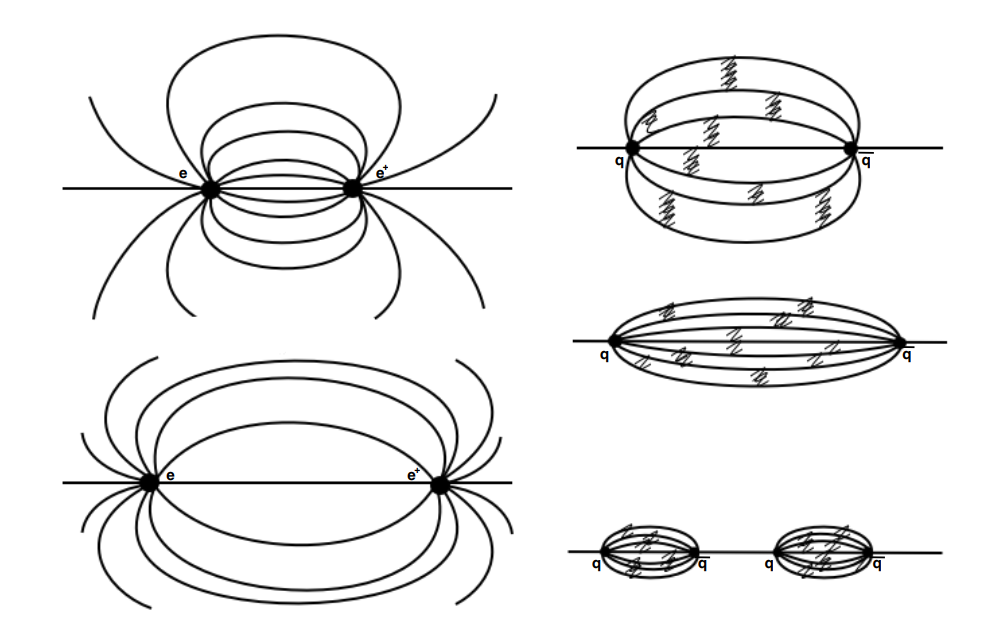
\includegraphics[width=0.7\textwidth]{figures/introduction/electric_color_fields.png}
    \caption{A schematic of the field lines between two electrically charged particles (left) and two quarks (right). The field lines between the quarks are pulled together due to the self-interaction of the gluons, whereas the electic field lines are not.}
    \label{fig:field_line_differences}
\end{figure}

\subsubsection{Asymptotic freedom}
\label{sec:qcd_asymptotic_freedom}

Just as the coupling constant becomes large at low energies and large distances, it also becomes small at high energies and small distances. This property is known as \textbf{asymptotic freedom}: at high enough energies, the quarks and gluons can be thought of as ``free'', and their interactions can be modeled using perturbative QCD (pQCD). As discussed in Section~\ref{sec:introduction}, the discovery of asymptotic freedom in QCD was what allowed for the accurate predictions of the results of high energy particle collision experiments like SLAC~\cite{SLAC} and PETRA~\cite{PETRA}. The results of such experiments have also been used to calculate the value of the coupling constant itself at different energy scales, as shown in Figure~\ref{fig:asymptotic_freedom}. The value of $\alpha_s$ at the Z$^0$ mass is also given in the figure, which is the most accurate measurement of $\alpha_s$ to date~\cite{PDG}. 

\begin{figure}
    \centering
    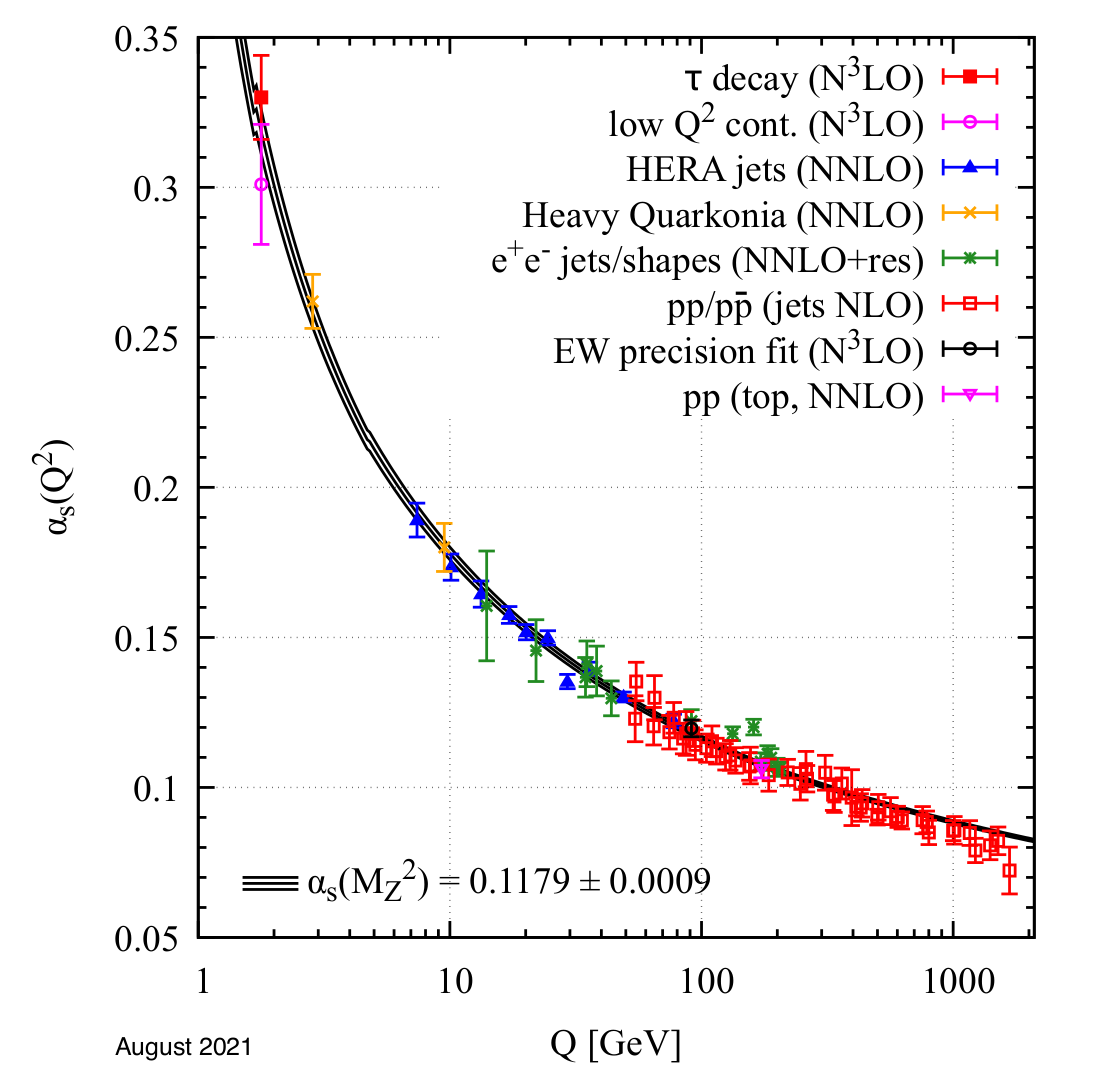
\includegraphics[width=0.7\textwidth]{figures/introduction/running_coupling.png}
    \caption{The value of the strong coupling constant $\alpha_s$ as a function of momentum transfer $Q$, which represents the energy scale of the interaction.}
    \label{fig:asymptotic_freedom}
\end{figure}


\subsubsection{Jets}
\label{sec:jets}

During high energy particle collisions (between two protons, for example), the consituent partons of the protons will sometimes scatter off each other in a way that converts most of their initial longitudinal momentum (along the collision axis) into transverse momentum. Such a scattering is often referred to as a \textbf{hard scattering}. Because the momentum transfer is large, the cross section of the parton-parton scattering is calculable using pQCD. Furthermore, branching processes of the high momentum partons--like gluon radiation--can also be calculated perturbatively. Eventually, however, the partons will lose enough energy such that their behavior can no longer be described using perturbative techniques.

Luckily, the aforementioned Lund model is well equipped to deal with lower energy partons. Under the Lund model, as these colored partons move away from each other, the force between them increases until there is enough energy to produce a quark-antiquark pair (as discussed in Section~\ref{sec:qcd_confinement}). This process--known as string fragmentation--continues until the partons are no longer energetic enough to move away from each other, at which point they hadronize into a large number of color neutral bound states. These hadrons are roughly collimated in the direction(s) of the initial hard scattering, forming sprays of particles that may end up being seen by a detector. These hadronic showers are known as \textbf{jets}. and they are one of the first experimentally observed predictions of QCD. A diagram depicting the formation of a jet from an initial hard scattering of partons can be seen in Figure~\ref{fig:jet_diagram}. 

\begin{figure}[ht]
    \centering
    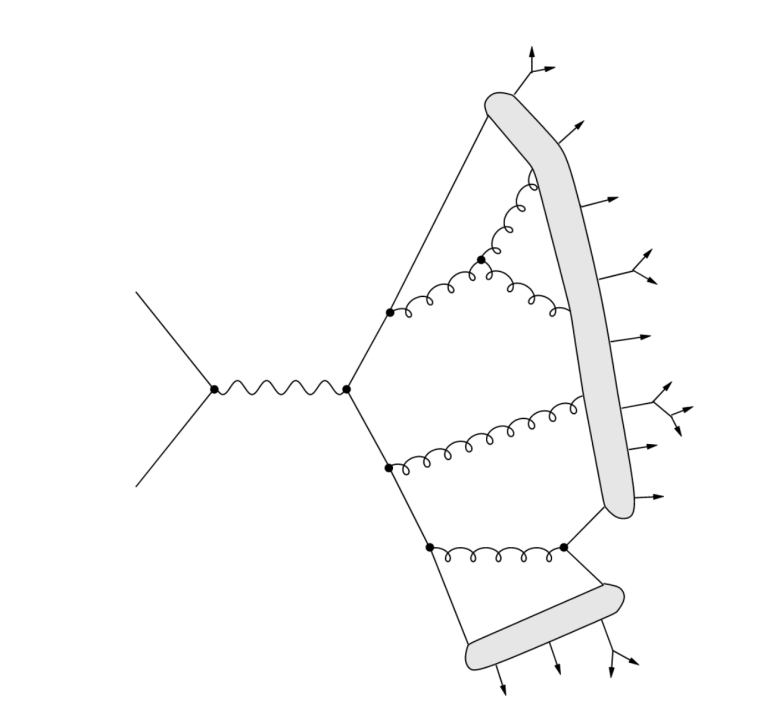
\includegraphics[width=0.7\textwidth]{figures/introduction/jet_string.png}
    \caption{A diagram depicting the formation of a jet within the Lund model from an initial hard scattering of partons, adapted from~\cite{JetStringDiagram}. The vertices represent perturbative QCD processes, the shaded regions represent string fragmentation/hadronization, and the outgoing arrows represent the resulting hadrons (which may decay further).}
    \label{fig:jet_diagram}
\end{figure}

Jets serve as a useful experimental probe to study the strong interaction: they combine the perturbative and non-perturbative regimes of QCD, and they are relatively easy to identify in a detector.

\subsection{The Quark-Gluon Plasma}
\label{sec:qgp}

One of the most exciting consequences of the asymptotic freedom of QCD is the existence of a new state of matter at extreme temperatures and densities: the \textbf{quark-gluon plasma} (QGP) ~\cite{QGP1, QGP2}. In this plasma, the quarks and gluons are not confined inside hadrons, and instead behave as quasi-free particles. This is analagous to an electromagnetic plasma, where electrons and protons are dissociated from their atoms. Studying the QGP and its formation is interesting for a number of reasons, but those reasons often get lost in the cosmological hype: the universe is thought to have been composed of this plasma in the first few microseconds after the Big Bang~\cite{QGP3}. Thus studying the QGP \textit{can} give insight to the early universe and its expansion, which is schematically represented in Figure~\ref{fig:qgp_universe}. 

\begin{figure}
    \centering
    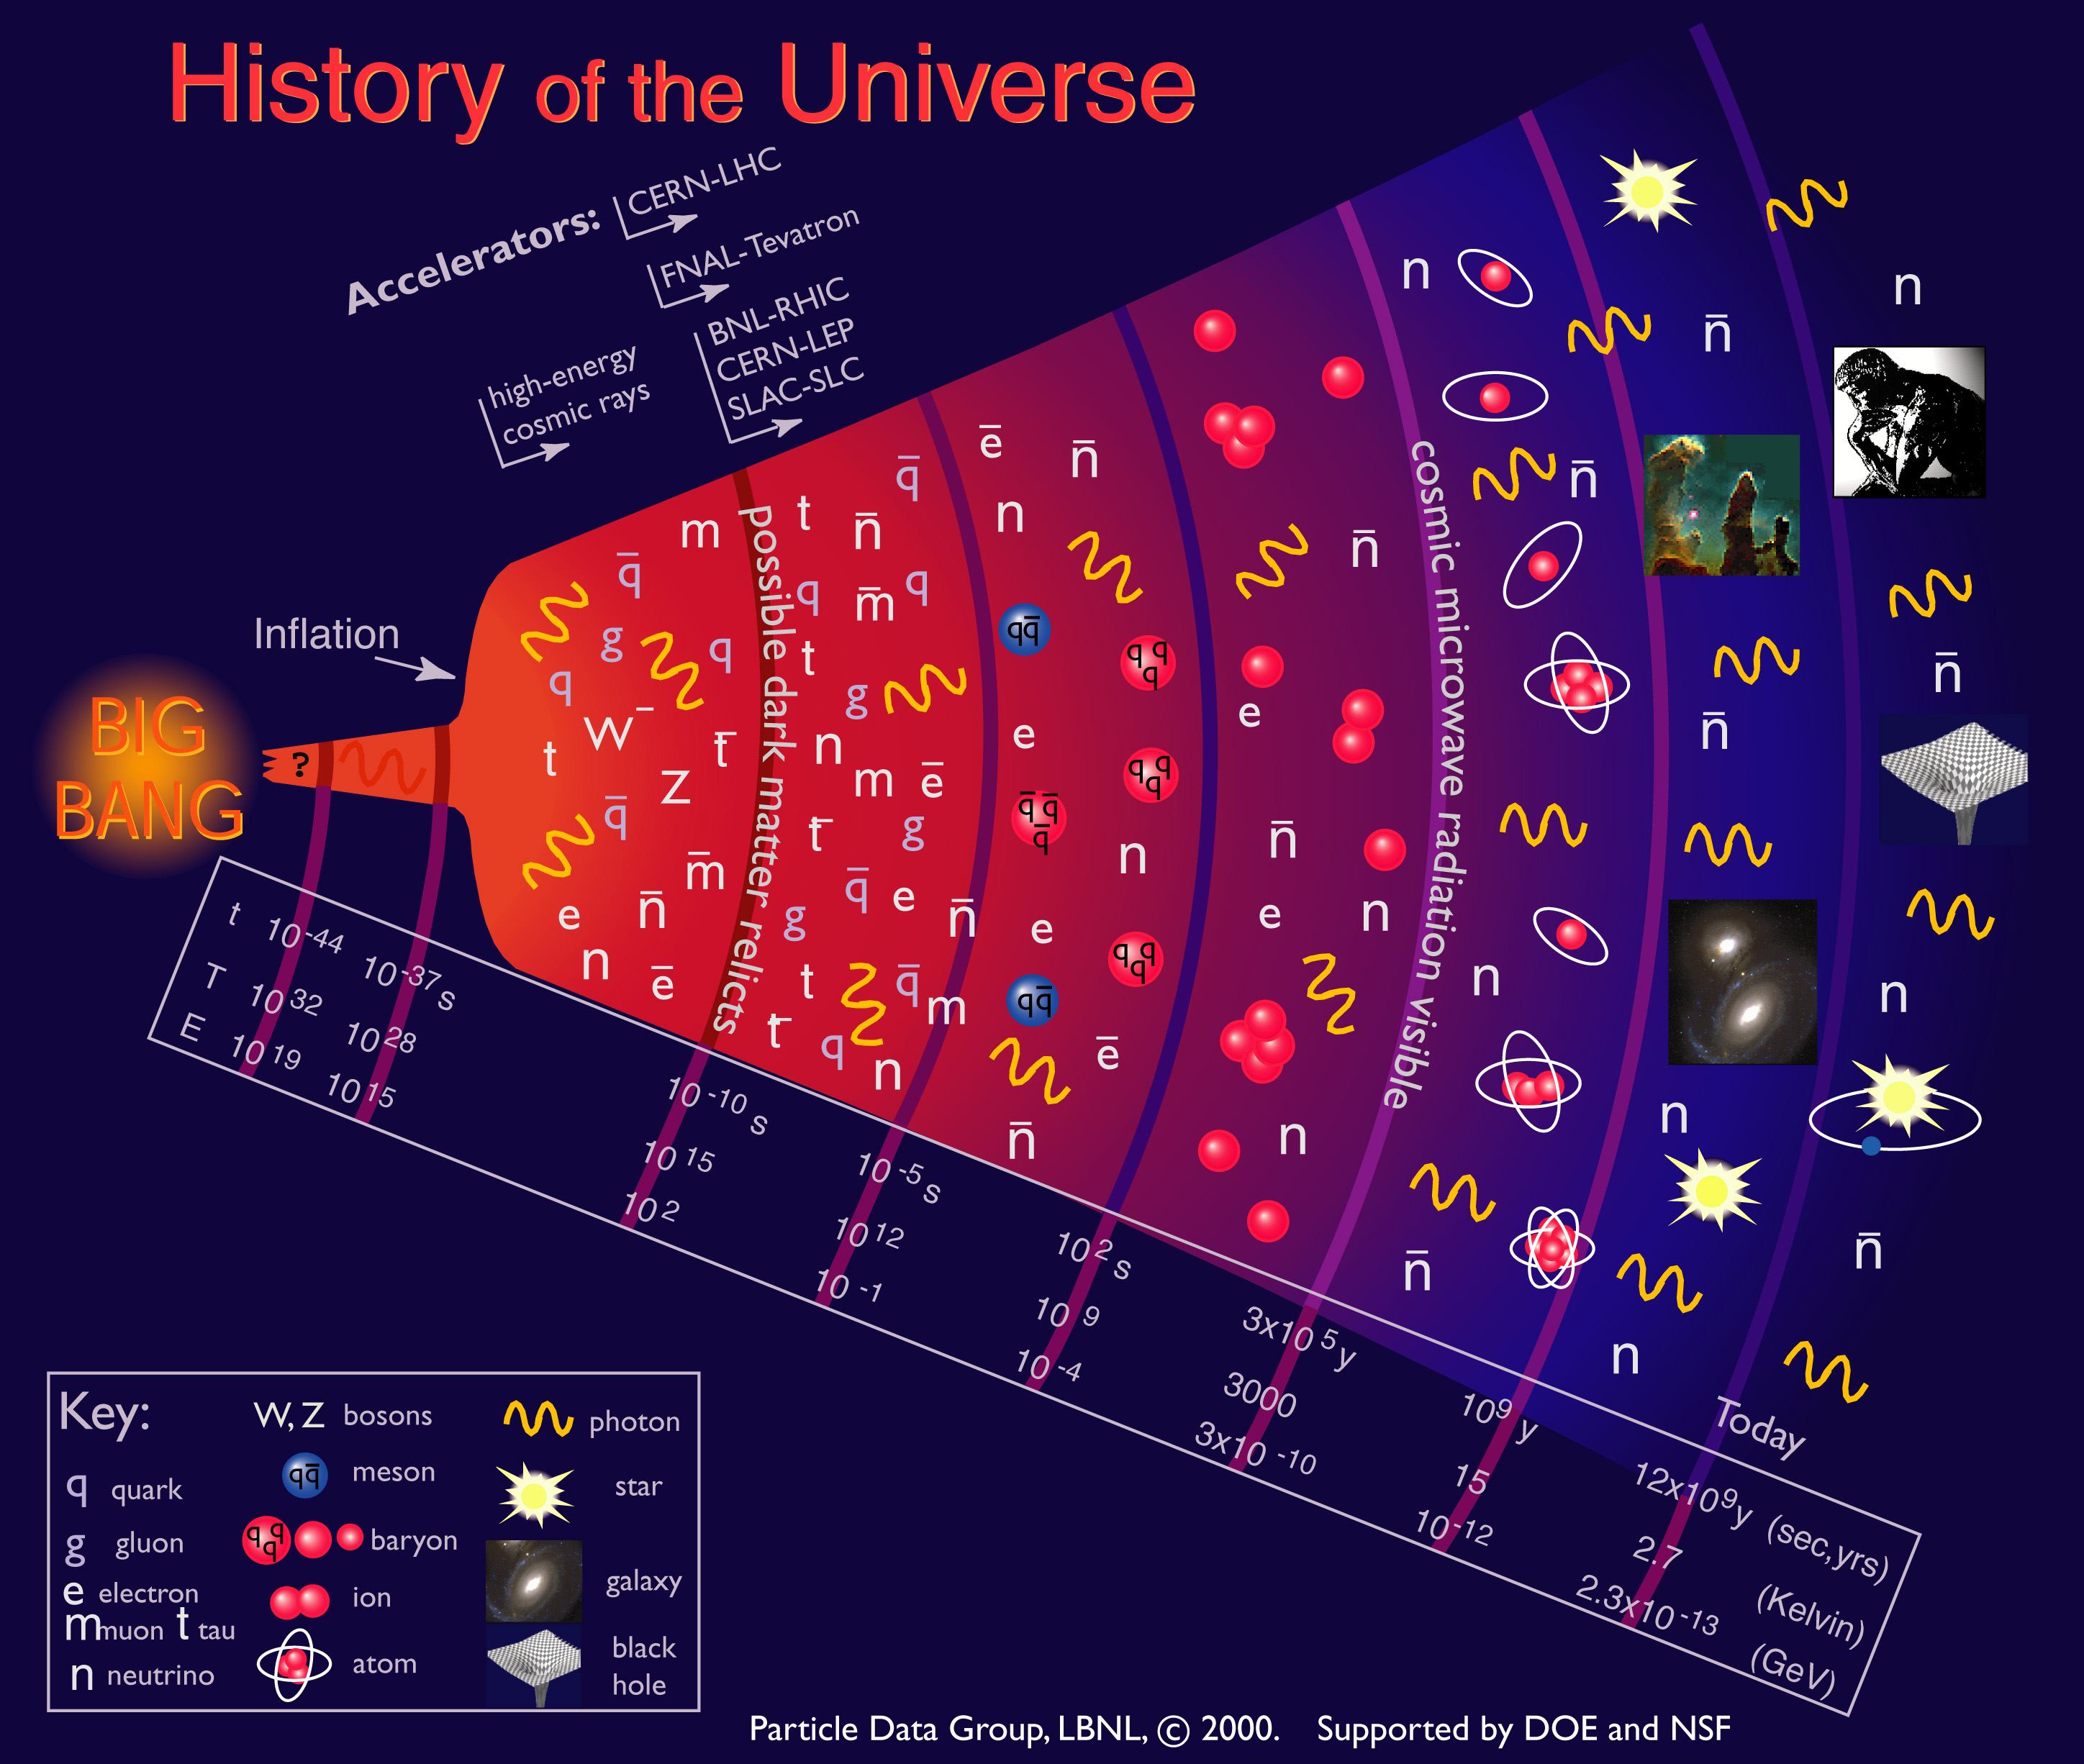
\includegraphics[width=0.7\textwidth]{figures/introduction/qgp_universe.jpg}
    \caption{A schematic of the evolution of the universe, taken from~\cite{QGPUniverse}. The QGP phase of the universe on this diagram lies roughly between 10$^{-10}$ and 10$^{-5}$ seconds after the Big Bang.}
    \label{fig:qgp_universe}
\end{figure}

However, the QGP is also very interesting from a purely particle physics perspective: it is a highly non-perturbative QCD system that can be generated in a laboratory setting. Studying this plasma and its properties can help illuminate the dark, confounding corners of QCD that are not yet understood--like confinement. Unfortunately producing this plasma in a laboratory setting is not a trivial task, and requires\footnote{There are hints of QGP formation in proton-proton collisions, which will be discussed in Section~\ref{sec:qgp_signatures}} colliding heavy ions at very high energies.


\section{Heavy ion collisions}
\label{sec:heavy_ion_collisions}

